\chapter{Hardwarebeschreibungssprachen - Hardware Description Language (HDL)}

\section{Allgemein}

\section{VHDL}
	
\subsection{Geschichte}
	VHDL - Very High Speed Integrated Circuit (VHSIC) Hardware Description Language
	
	\begin{description}
		\item[1981] Initiert durch US Verteidigugnsministerium um die Wiederverwendung von Hardware in neuen Technologien zu vereinfachen
		\item[1983] Intermetrics, IBM and TI wollen eine ADA-basierte HDL entwerfen
		\item[1985] Vollendung des VHDL-Core in Version 7.2
		\item[1986] US Verteidigugnsministerium übergibt alle Rechte an VHDL an IEEE
		\item[1987] VHDL wird IEEE-Standard 1076-1987
		\item[1987] US Verteidigugnsministerium benötigt VHDL-Modelle für alle eingekauften ASICs
		\item[1988] VHDL wird ANSI-Standard
		\item[1993] IEEE-Standard 1076-1993 ist immer noch weitv erbreitet
		\item[2008] IEEE-Stanard 1076-2008 letzte Hauptversion von VHDL
	\end{description}
	
\subsection{Abstraktionsebenen}
	VHDL ist geeignet folgende Ebenen zu beschreiben:
	\begin{itemize}
		\item Systemebene
		\item Algorithmische Ebene
		\item Register-Transfer-Ebene (RTL)
		\item Logikebene (gate level)
	\end{itemize}
	\begin{center}
		\includegraphics[page=4, width=0.8\linewidth, trim=10mm 30mm 10mm 32mm, clip]{\Path/resources/Vorlesung/VLSI/04_vhdl.pdf}
	\end{center}
	
\subsection{Grundsätze}
	\paragraph{Struktur}\hfill\\
	Entwürfe werden aus Komponenten zusammengebaut.\\
	\begin{center}
		\includegraphics[page=6, width=0.8\linewidth, trim=10mm 30mm 10mm 40mm, clip]{\Path/resources/Vorlesung/VLSI/04_vhdl.pdf}
	\end{center}
	\begin{itemize}
		\item typischerweise: weite, bidirektionale Schnittstellen (Drähte)
		\item hierarchischer Instanzierungsbaum der Komponenten
		\item Verdrahtung in oder durch Instanziierungs-Modul
	\end{itemize}
	
	\paragraph{Kohärenz}
	Implementierungen werden aus kohärenten Aussagen gebildet.
	\begin{itemize}
		\item Reihenfolge der Aussagen ist unwichtig\\
			\(p <= a\, xor\, b;\\s <= p\, xor\, c;\)\\
			ist äquivalent zu\\
			\(s <= p\, xor\, c;\\p <= a\, xor\, b;\)
		\item Abhängigkeiten werden durch Signalverbindungen definiert!
	\end{itemize}
	
\section{Verilog}

